\documentclass[11pt,a4paper]{article}

\usepackage[ngerman]{babel}
\usepackage[utf8]{inputenc}
\usepackage[T1]{fontenc}
\usepackage{lmodern}
\usepackage{amsmath}
\usepackage{graphicx}
\usepackage{float}
\usepackage{hyperref}

\title{Reinforcement Learning - Übung 02}
\author{Gruppe 4 - Amos Mohr, Daniel Maier, Sifan Zhu, Tommy Kiss}
\date{\today}

\begin{document}

\maketitle

\section*{1)}
Siehe Implementierung!
\section*{2)}
Siehe Implementierung!
\section*{3)}
\subsection*{3.1)}
\begin{figure}[H]
    \centering
    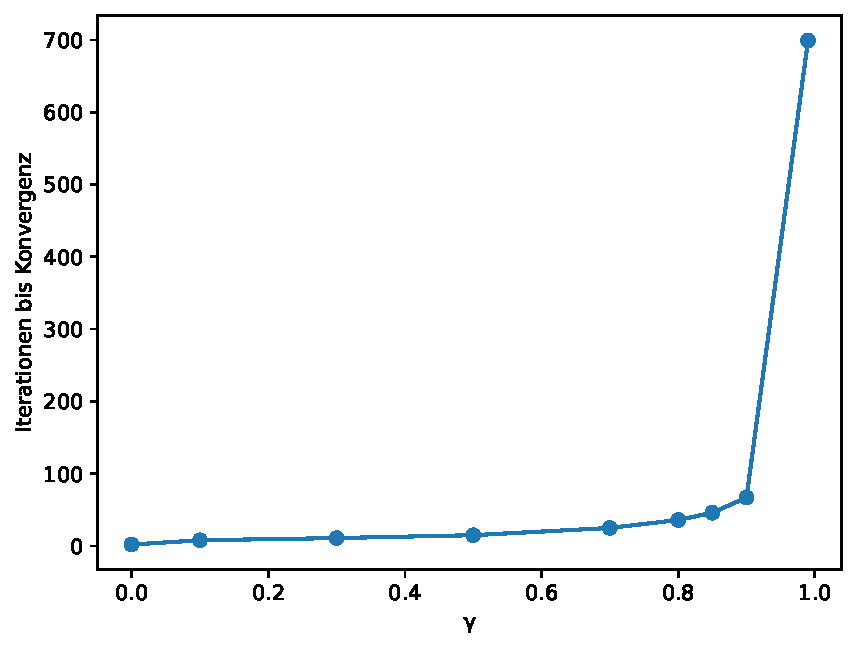
\includegraphics[width=0.8\textwidth]{plot-31.pdf}
\end{figure}
Für kleine Werte von $\gamma$ konvergiert das Verfahren also viel schneller, insgesamt einigermaßen stabil bis inklusive $\gamma = 0.85$ und danach Zusammenbruch der Konvergenzgeschwindigkeit.
Intuitiv macht es Sinn, da bei höherem $\gamma$ die Iteration weitsichtiger ist, es werden weiter in der Zukunft liegende Zustände mit gewichtet.
Es geht also immer weniger um den unmittelbaren reward und immer mehr um den langfristig kumulierten reward.
\subsection*{3.2)}
\begin{figure}[H]
    \centering
    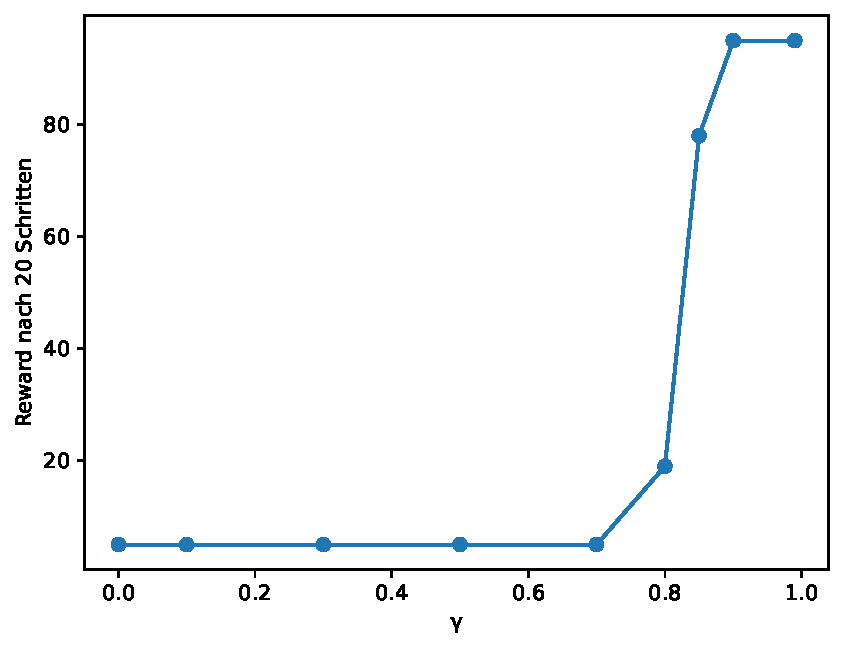
\includegraphics[width=0.8\textwidth]{plot-32-1.pdf}
\end{figure}
Man sieht, dass die größten beiden Werte für $\gamma$ auch den größten Reward nach 20 Schritten liefert.
Intuitiv macht das Sinn:
Größeres $\gamma$ $\Rightarrow$ langsamere Konvergenz $\Rightarrow$ insgesamt mehr über die wahre value-Funktion gelernt.
\subsection*{3.3)}
Wenn es um die Frage geht, welcher Wert für Gamma im Bezug auf die investierte Rechenleistung und den gewonnenen Reward das beste Preis-Leistungsverhältnis hat, lässt sich dies am einfachsten anhand eines Scores $\text{score} = \frac{\text{reward}}{\text{iteration}}$ abbilden:
\begin{figure}[H]
    \centering
    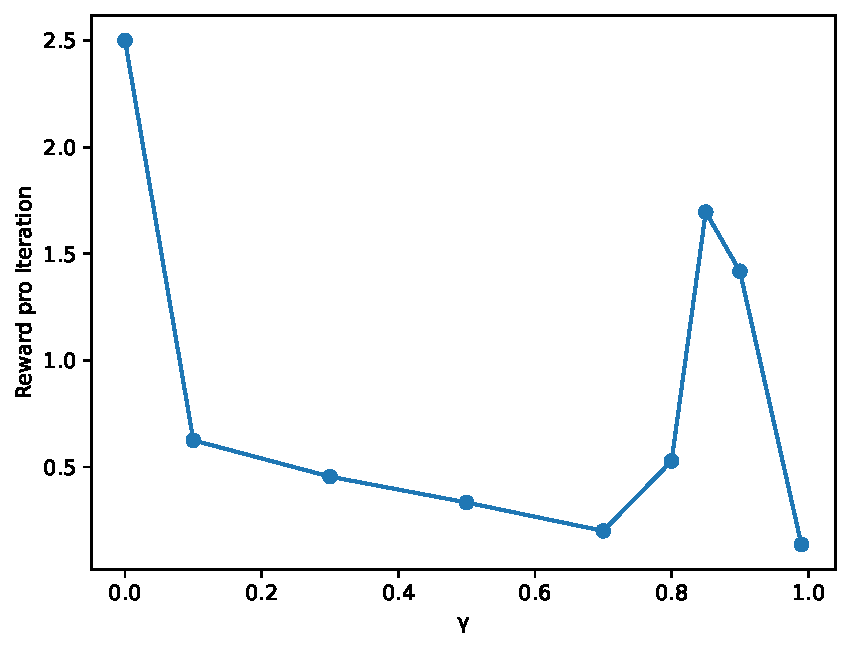
\includegraphics[width=0.8\textwidth]{plot-32-2.pdf}
\end{figure}
Man sieht, dass für $\gamma = 0.1$ der beste score entsteht, d.h. in diesem Fall ist das beste Preis-Leistungsverhältnis gegeben.
\section*{4)}
Wir haben es nicht ersetzt sondern neu implementiert, siehe Zelle mit Aufgabe 4.
Dort werden die nötigen Parameter konstruiert, die Funktion aufgerufen und das policy-Objekt so rekonstruiert, dass wir es plotten können.
Abgesehen davon, dass die Übergabeformate abweichen, muss man hauptsächlich ein Objekt zusätzlich übergeben, dass die Transitionswahrscheinlichkeiten modelliert.
Diese sind bei uns implizit und stehen in der ValueIteration Funktion.
Wir verwenden den Spezialfall, dass alle Transitionen deterministisch sind, also ist die entstehende Matrix (pro Aktion) eine Matrix mit einer 1 und sonst nur 0en in jeder Zeile.
Man sieht, dass die gefundene Policy die gleiche ist.
\section*{5)}
\begin{figure}[H]
    \centering
    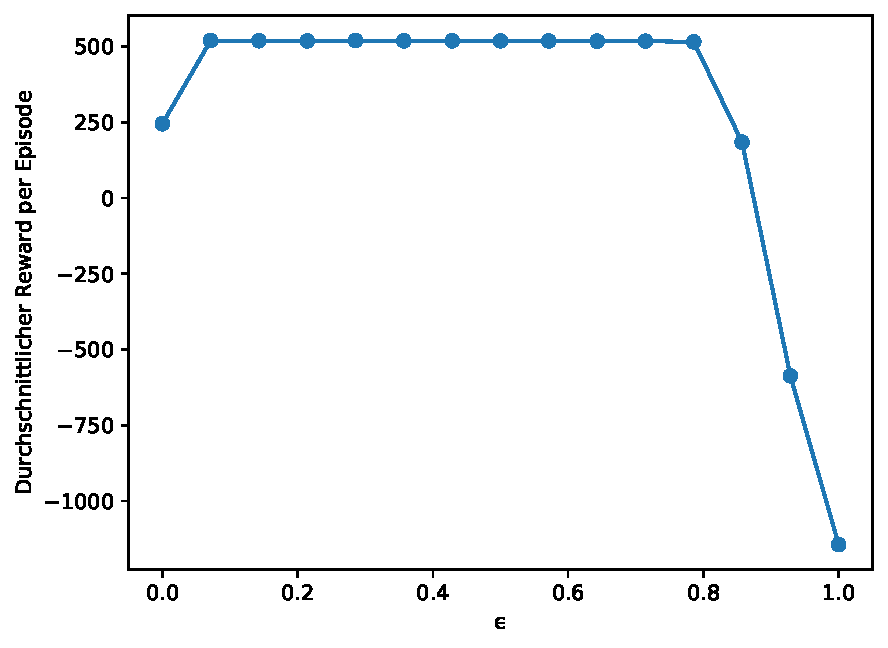
\includegraphics[width=0.8\textwidth]{plot-5-1.pdf}
\end{figure}
\begin{figure}[H]
    \centering
    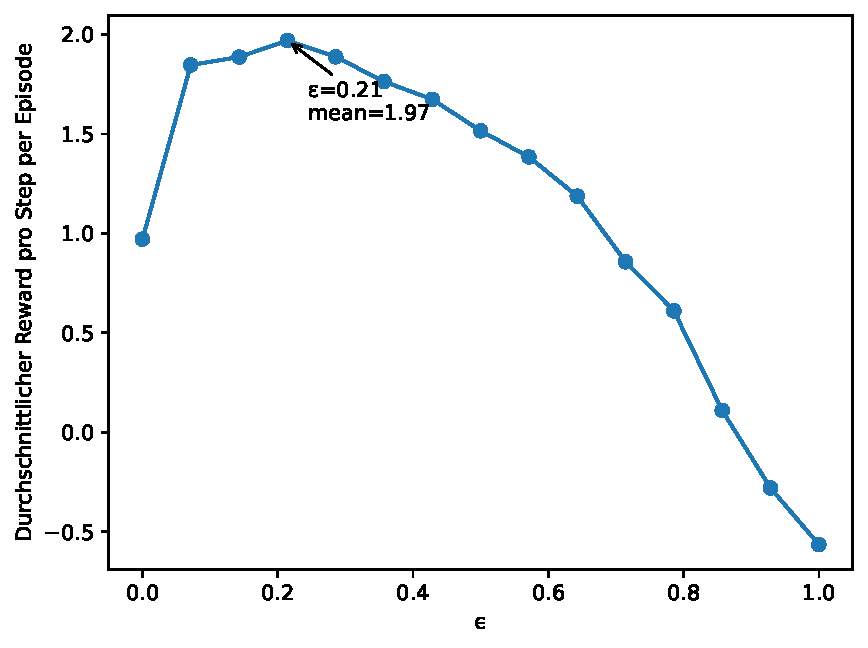
\includegraphics[width=0.8\textwidth]{plot-5-2.pdf}
\end{figure}
Man sieht hier eine Darstellung der durchschnittlichen Rewards per Episode sowie der Rewards pro Step, per Episode über je 100 Episoden mit 2000 Steps und $\gamma = 0.9$, in Abhängigkeit von $\epsilon$.
Offenbar ist der durchschnittliche Reward relativ unempfindlich gegen den Parameter $\epsilon$, solange er nicht extrem am Rand des Intervalls liegt und ungefähr $\leq 0.85$ ist.
Beim Reward pro Step zeigt sich dagegen eine klare Präferenz für kleine Werte $\ge 0.07$, mit einem Maximum bei $0.07$ mit durchschnittlichem Reward pro Step von $1.91$.

\end{document}
